\documentclass{article}
\usepackage{graphicx}
\usepackage{lmodern} % Fix the font size warnings
\usepackage{fancyhdr} % Required for custom headers
\usepackage{lastpage} % Required to determine the last page for the footer
\usepackage{extramarks} % Required for headers and footers
\usepackage{graphicx} % Required to insert images
\usepackage{xfrac} % Nice fractions
\usepackage{amsmath}

\usepackage{multicol}

% Margins
\topmargin=-0.5in
\evensidemargin=0in
\oddsidemargin=-0.5in
\textwidth=7.5in
\textheight=9.0in
\headsep=0.25in 

% paragraphs
\usepackage{parskip}

\pagestyle{fancy}

\rhead{Main courses}
\lhead{\textbf{Dads's Meatballs}}
\chead{}
\title{Dad's Meatballs}

\begin{document}
Ok, this one takes a bit of work. But, really, it's worth it. Best to make the meatballs and the matching sauce in one
go because it's a lot. This makes about 40 meatballs or something.

\begin{multicols}{2}

      \textbf{Meatballs}
      \begin{itemize}
            \item 3 16 ounce packages of ground turkey
            \item 2 16 ounce packages of Italian turkey sausages
            \item 2 16 ounce packages of turkey breakfast sausage
            \item 1 bunch Italian parsley (about 1 cup)
            \item 1 bunch basil (about 4 tablespoons chopped)
            \item 3 cups Italian white bread, crust removed and diced
            \item 1 cup whole milk
            \item 3 eggs
            \item 1 medium shallot
            \item \sfrac{1}{2} head of garlic (about 8 to 10 cloves)
            \item 2 tablespoons red pepper flakes
            \item 2 teapoons salt
            \item 2 teapoons pepper
      \end{itemize}

      \columnbreak

      \textbf{Sauce}
      \begin{itemize}
            \item 2 32 ounce cans of crushed tomatoes
            \item 1 32 ounce can of tomato sauce
            \item 1 32 ounce can of diced tomatoes
            \item 3 tablespoons olive oil
            \item 3 medium shallots, diced
            \item \sfrac{1}{2} head of garlic (about 8 to 10 cloves)
            \item 1 bunch basil, (about 4 tablespoons chopped)
            \item 2 tablespoons red pepper flakes
            \item 1 tablespoon salt
            \item 1 tablespoon pepper
      \end{itemize}

\end{multicols}

\textbf{The meatballs}

Start by soaking the diced bread in the cup of milk for at least 10 minutes. You want the bread to be
soft and nearly falling apart. While the bread is soaking coursely chop the shallots, garlic, basil,
and parsley, and put them into a food processor.  Add the garlic and shallots to the food processor.
When the bread is ready, squeeze a bit of the milk out, add \sfrac{1}{2} of it and \sfrac{1}{2} pound
of the ground turkey to the food processor and process until most of ``those green thingies'' are
ground up and no longer really visible. Remove the turkey from the food processor to a large bowl, add the
remaining bread and another \sfrac{1}{2} pound of ground turkey.

Peel the Italian sausages by slicing them lengthwise and removing the casing. Put the peeled sausages,
breakfast sausage, remaining turkey, salt, pepper, and two eggs into a very large bowl. Scrap the turkey
from the food processor into the bowl. Now, smoosh it all together until everything is evenly mixed.

Spray two large jelly roll pans with PAM. Measure 3\sfrac{1}{2} ounce portions of the meat and form them
into firm balls. Place these on the jelly roll pans. You'll end up filling both of the pans. When you're done
making the meatballs put them in a 425 degree oven until they are cooked on the outside and read around
165 degrees with an instant-read thermometer.

\textbf{The sauce}

While the meatballs are baking heat the olive oil over a medium flame in a very large heavy bottomed Dutch oven.
I prefer the the 4 gallon All Clad for this. Add the shallot and garlic and cook until fragrant and the shallots
and garlic are translucent. Add the tomatoes starting with the diced ones (to reduce splashing). Add the remaining
ingredients. Fill one of the 32 ounce tomato cans with warm water and add to the pot.

\textbf{Putting it all together}

When the meatballs are done add them to the pot one at a time. Turn the sauce down to low-medium and let simmer
for 2 or 3 hours. Make sure to stir about every 15 minutes to keep the sauce from burning and to make sure all the
meatballs get a chance to cook under the sauce. You might need to keep adding water if the sauce starts to get too
thick.


% \begin{figure}
%     \centering
%     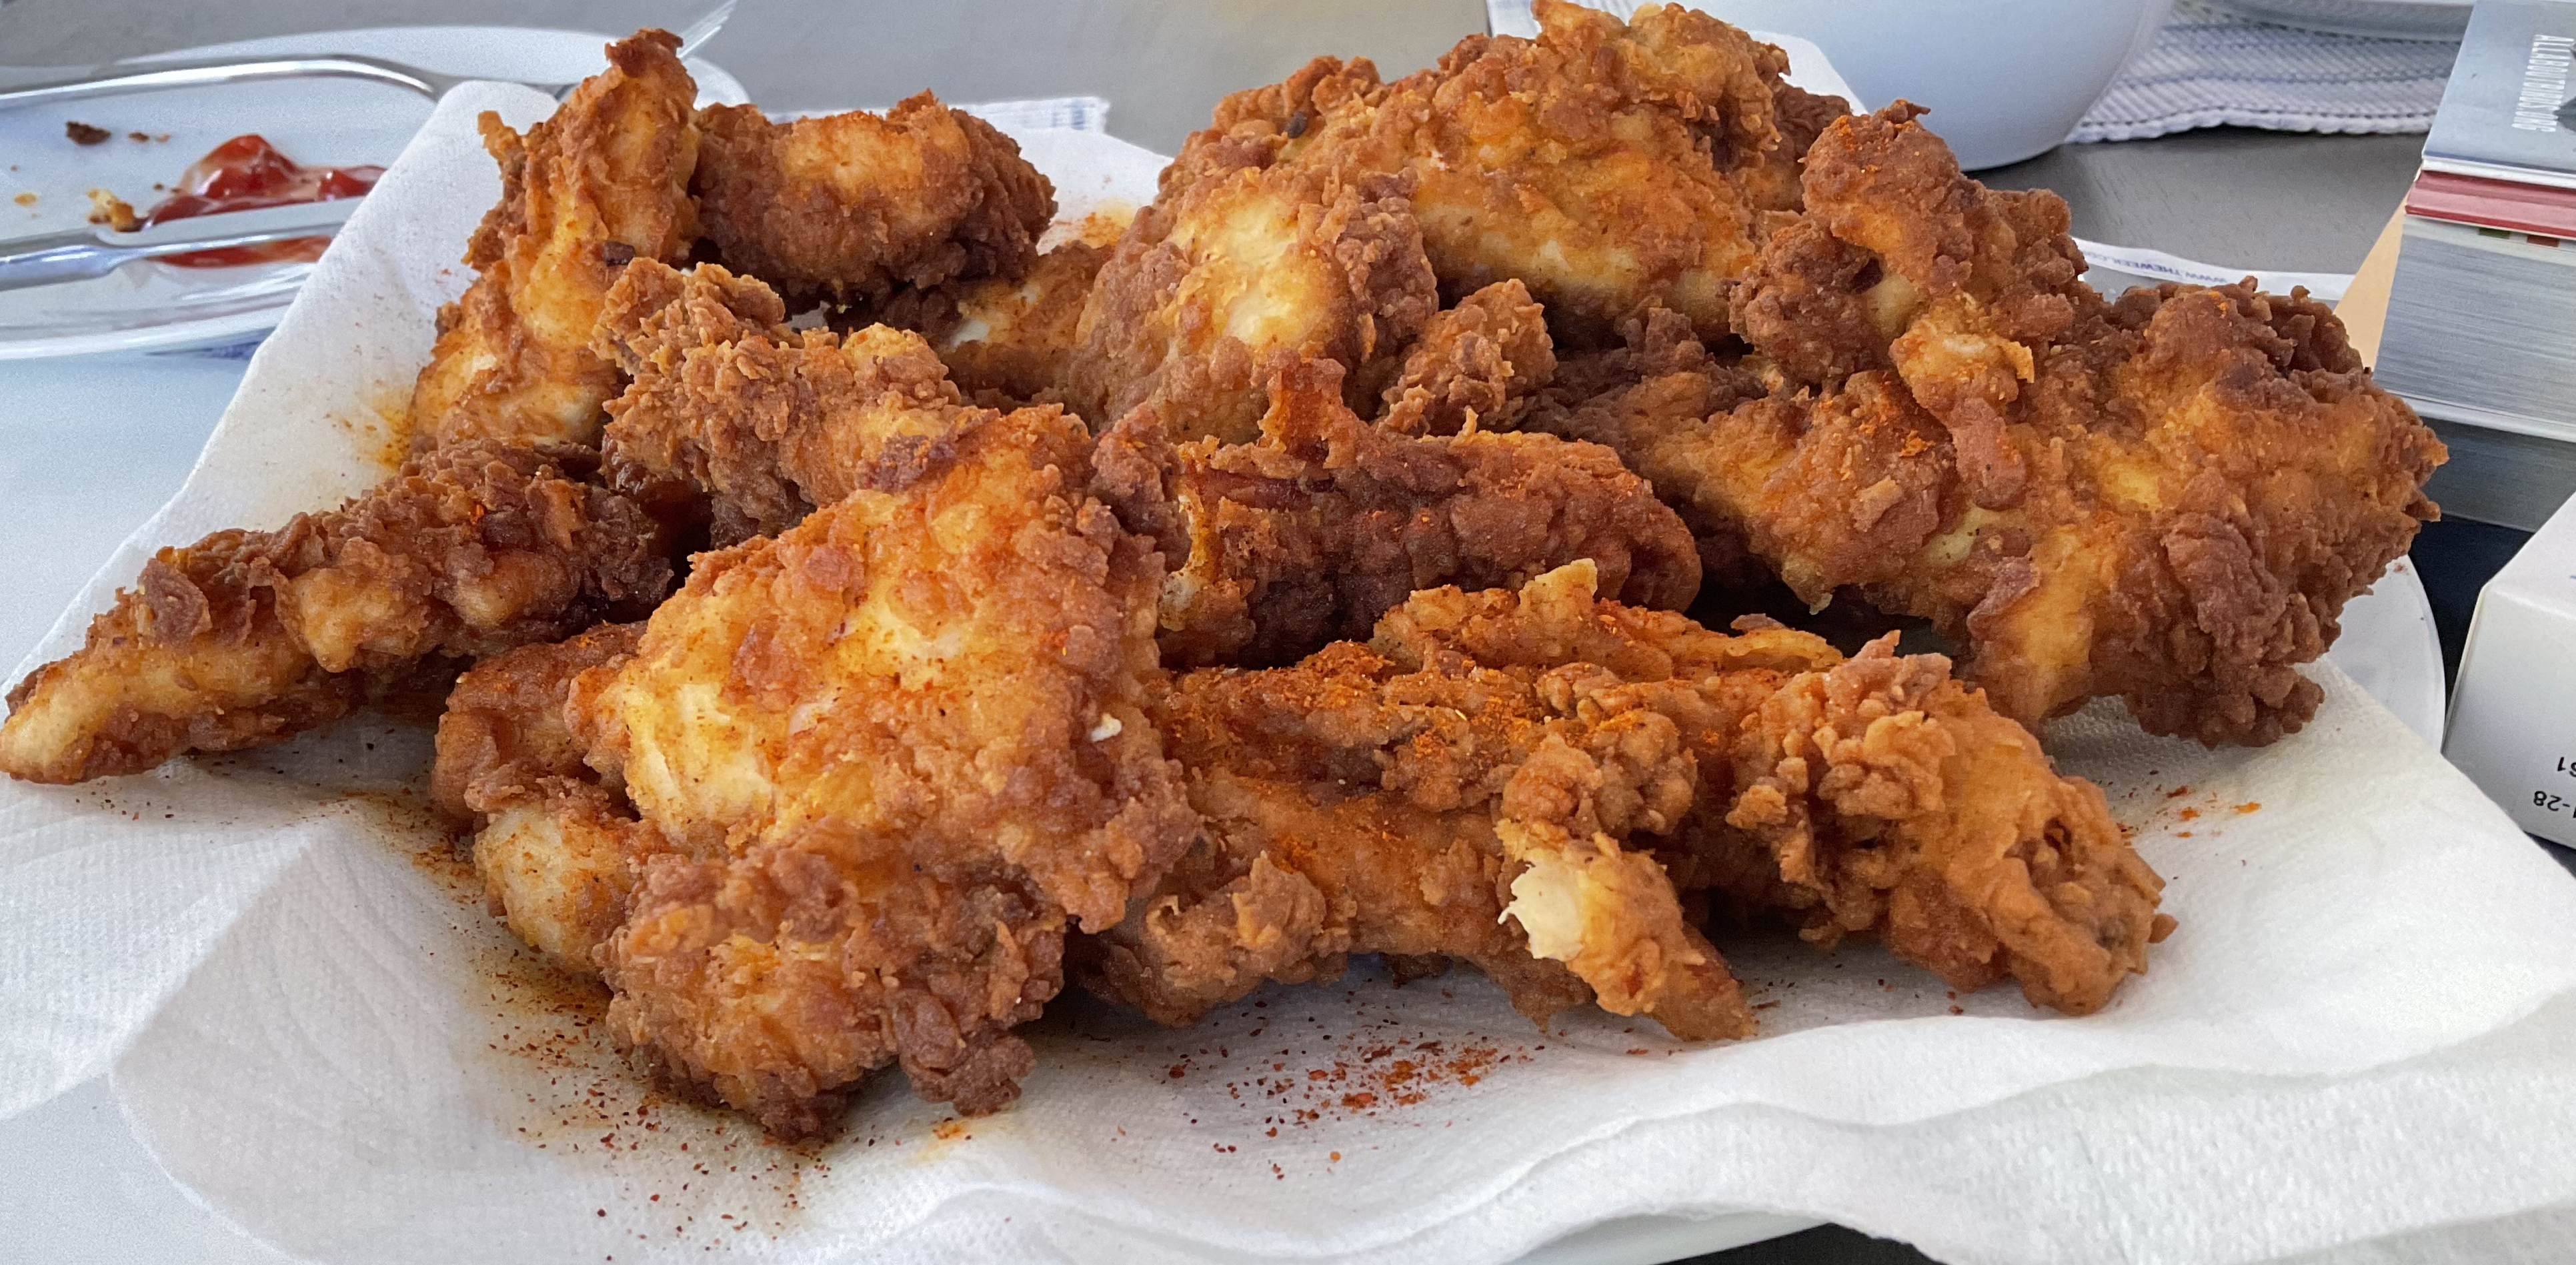
\includegraphics[scale=0.095]{fried-chicken.png}
% \end{figure}

\end{document}
